%In this section, we present our study results by answering our research questions. For each question, we discuss the motivation behind it, the approach to answering it and finally the results obtained. 
%\\
%
%\noindent\textbf{RQ1:} \textbf{How much do logs change over time and why do the changes occur?}
%\\

%\noindent\textbf{Motivation}

%Research has shown that logs evolve along with the code~\cite{IanContextinformation}. When logs are changed, the log  processing tools which are dependent on them also have to get updated. This results in costly maintenance effort. To understand the cost, we have to understand how frequent changes to logs are. Hence, we explore the frequency of changes to logs in our studied systems and why they are changed.\\

%\noindent \textbf{Approach}


%\begin{table*}
%	\centering
%	\caption{Distribution of log changes in different projects}
%	\label{tba:logchangeDistribution}
%	\begin{tabular}{l|>{\centering}p{.1\columnwidth}>{\centering}p{.01\columnwidth} 
%			p{0.01\columnwidth} }
%		\cline{1-4}  	\multicolumn{1}{|c}{Projects}    & \multicolumn{1}{|c}{Never Changed (\%) }  &  \multicolumn{1}{|c}{Changed (\%) }	   &  \multicolumn{1}{|c}{Frequently Changed (\%) }\\ \cline{1-4}   
%		
%		Life Ray      & 78.67     & 19.66 & 1.66           \\
%		
%		Camel      & 55.43    & 37.32 & 7.25            \\
%		ActiveMq   & 34.78     & 62.02 & 3.20           \\
%		CloudStack & 19.68     & 68.61 & 11.71          \\ \cline{1-4}
%	\end{tabular}
%\end{table*}

%\begin{table*}
%	\centering
%	\caption{Distribution of log changes in different projects}
%	\label{tba:logtype}
%	\begin{tabular}{l|llll}
%		\cline{1-5}  	\multicolumn{1}{|c}{Projects}    & \multicolumn{1}{|c}{ ActiveMQ }  &  \multicolumn{1}{|c}{ Camel}	   &  \multicolumn{1}{|c}{ Cloudstack }  & 
%		\multicolumn{1}{|c|}{ Liferay } \\ \cline{1-5}   
%		
%		Log relocation (\%)       & 20.05     & 20.80 &  53.32  & 49.42         \\
%		
%		Log text change (\%)      & 26.59    & 26.37 & 15.54    & 32.70       \\
%		Log variable change (\%)   & 53.18     & 52.75 & 31.08 &  16.75     \\
%		Change of log level (\%) & 0.18   & 0.08 & 0.04  &  1.13       \\ 
%%		Text and variable change (\%) & 2.33     & 6.39 & 22.0   &  30.59    \\ 
%\cline{1-5}
%	\end{tabular}
%\end{table*}


%In this paper we aim to get a better understanding of the
%unstable logs in an project so that we can improve the maintenance of log processing tools. 
<<<<<<< HEAD
In this paper we study the changes that are made to logging statements in open source projects. The goal of our study is to present a classifier for deciding whether a logging statement is likely to change in the future. This classifier can assist developers of log processing tools in deciding on which logging statements they want their tool to depend. %In order to understand and build a random forest classifier to predict log changes, it is necessary to identify the extent logs are changed within these projects.
First, we perform a preliminary analysis, in which we examine how often logging statements change, to motivate our work. In this section, we present our rationale for selecting the projects that we studied and present the results of our preliminary analysis of the four studied projects. 
=======
In this paper we study the changes that are made to logging statements  in open source applications. The goal of our study is to present a classifier for deciding whether a logging statement is likely to change in the future. This classifier can assist developers of log processing tools to decide on which logging statements they want their tool to depend. %In order to understand and build a random forest classifier to predict log changes, it is necessary to identify the extent logs are changed within these projects.
First, we perform a preliminary analysis, in which we examine how often logging statements change, to motivate our work. In this section, we present our rationale for selecting the applications that we studied and present the results of our preliminary analysis of the four studied applications. 
>>>>>>> c81afe5aab4af1198487f4494a3314e260e9fd43

\subsection{Studied Applications}
We selected our studied applications based on the following three criteria:
\begin{itemize}
<<<<<<< HEAD
	\item \textbf{Usage of logging statements.} The projects must make extensive use of logging statements in their source code.
	%	This helps to improve the performace of the random forest classifier and to identify the factors which effect log stability.
	\item \textbf{Project activity.} The projects must have a mature development history (i.e., more than 10,000 commits).
	\item \textbf{Technology used.} To simplify the implementation of our study, we opted to only select projects that are written in Java and are available through a Git repository.
=======
	\item \textbf{Usage of logging statements} - The applications must make extensive use of logging statements in their source code
	%	This helps to improve the performace of the random forest classifier and to identify the factors which effect log stability.
	\item \textbf{Application activity} - The applications must have a mature development history (i.e., more than 10,000 commits)
	\item \textbf{Technology used} - To simplify the implementation of our study, we opted to select only applications that are written in Java and are available through a Git repository
>>>>>>> c81afe5aab4af1198487f4494a3314e260e9fd43
%	We pick projects written in Java as it is one of the most popular languages today~\cite{Javaprog}.
%	 to identify and track the log changes across multiple releases. 
\end{itemize}

<<<<<<< HEAD
To select projects that match these criteria, we first selected all Java projects from the list of Apache Foundation Git repositories\footnote{\url{https://git.apache.org/}} that have more than 10,000 commits. Next, we counted the number of logging statements in all \code{*.java} files in a repository using the \code{grep} command in Listing~\ref{lst:grep}.
=======
To select applications matching these criteria, we first selected all Java applications from the list of Apache Foundation Git repositories\footnote{\url{https://git.apache.org/}} that have more than 10,000 commits. Next, we counted the number of logging statements in all \code{*.java} files in a repository using the \code{grep} command in Listing~\ref{lst:grep}.
>>>>>>> c81afe5aab4af1198487f4494a3314e260e9fd43

\vspace{-5mm}
\begin{Code}
\begin{lstlisting}[caption={Counting logging statements}, label={lst:grep}]
grep -icR 
"\(log\.*\)\.\(|info\|trace\|debug\|error\|warn\)(" . 
| grep "\.java"
\end{lstlisting}
\end{Code}
\vspace{-5mm}

This command counts the occurrences in a file of an invocation of a logging library (e.g., \code{log} or \code{\_logger}) followed by the specification of a log level. We sum the occurrences in all files of an application to get the total number of logging statements shown in Table~\ref{tba:overviewsystems}.
%To find the log usage in an project we use the \emph{grep} command to search all lines of code within the \emph{.java} files. %Next, using \emph{git log} we find the total number of commits in the code repositories and select projects which have more than 10,000 commits.
 
We select the four applications (ActiveMQ, Camel, Cloudstack and Liferay) with the highest number of logging statements for further analysis. ActiveMQ\footnote{\url{http://activemq.apache.org/}} is an open source message broker and integration patterns server. Camel\footnote{\url{http://camel.apache.org/}} is an open source integration platform based on enterprise integration patterns. CloudStack\footnote{\url{https://cloudstack.apache.org/}} is an open source application designed to deploy and manage large networks of virtual machines. Liferay\footnote{\url{http://www.liferay.com/}} is an open source platform for building websites and web portals. Table~\ref{tba:overviewsystems} presents an overview of the studied applications. %We pick the releases after incubation for each project, as during incubation the projects might not be used by log processing tools.  


\begin{table}[tb]
	\centering \protect\protect\caption{An overview of the studied applications (all metrics calculated using the latest HEAD of the repository) }
	\smaller
	\newcolumntype{R}[1]{>{\raggedleft\arraybackslash}m{#1}}

	\label{tba:overviewsystems} %

	
	\begin{tabular}{>{}p{3cm}R{1.0cm}R{.7cm}R{1.1cm}R{1.0cm}}
		\toprule 
		~ & \textbf{ActiveMQ}  & \textbf{Camel}  & \textbf{CloudStack}  & \textbf{Liferay} \\
		\midrule
		\# of logging statements & 5.1K  & 6.1K & 9.6K  & 1.8K \\
		\# of commits &	 11K  & 21K  & 29K  & 143K \\	
		\# of years in repository&	 8  & 8  & 4  & 4 \\
		\# of Contributors&41&151&204&351\\
%		\# of releases  & 19  & 43  & 111  & 24 \\
		\midrule
		\# of added lines of code  & 261K  & 505K  & 1.09M  & 3.9M \\
		\# of deleted lines of code  & 114K  & 174K  & 750K  & 2.8M \\
		\# of added logging statements  & 4.5K  & 5.1K  & 24K  & 10.4K \\
		\# of deleted logging statements  & 2.3K & 2.4K  & 17K  & 8.1K \\
		\% of logging-related changes & 1.8\% & 1.1\% & 2.3\% & 0.3\% \\

		\bottomrule 
	\end{tabular}
	\vspace{-0.3cm}
\end{table}

\subsection{Data Extraction Approach}

The data extraction approach from the four studied applications consists of three steps, which are explained further in this section: 

\begin{enumerate}
<<<<<<< HEAD
\item We clone the Git repository of each studied project in order to extract the change history of each file.
\item We identify the logging statements in the repository.%, and use the change history to identify changes made to these logging statements
\item We track the changes that are made to each logging statement across commits.
=======
\item We clone the Git repository of each studied application in order to extract the change history of each file 
\item We identify the logging statements in the repository%, and use the change history to identify changes made to these logging statements
\item We track the changes that are made to each logging statement across commits 
>>>>>>> c81afe5aab4af1198487f4494a3314e260e9fd43
\end{enumerate}

We use R~\cite{ihaka1996r} to perform our preliminary analysis. Figure~\ref{fig:LGmethod} shows a general overview of our approach and we detail below each of the aforementioned steps. 

\subsubsection*{B.1. Extracting the change history of Java files} 
%In order to find the stability of logs, we have to identify all the Java files in our studied projects. To achieve this, we use the \emph{grep} command to search for all the \emph{*.java} files in the cloned repositories and we exclude the \emph{test} files. 
<<<<<<< HEAD
To examine the changes that are made to logging statements, we must first obtain a complete history of each Java file in the latest version of the main branch.
We collect all the Java files in the four studied projects and we use their Git repositories to obtain all the changes that are made to the files. We use Git's \emph{follow} option to track a file even when it is renamed or relocated. We include only the changes to logging statements that are made in the main branch as other logging statements are unlikely to affect log processing tools. %We use the \emph{--no-merges} option to flatten the changes to a file and exclude the final merging commit. 
=======
To examine the changes made to logging statements, we must first obtain a complete history of each Java file in the latest version of the main branch.
We collect all the Java files in the four studied applications and we use their Git repositories to obtain all the changes that are made to the files. We use Git's \emph{follow} option to track a file even when it is renamed or relocated. We include only the changes to logging statements that are made in the main branch as other logging statements are unlikely to affect log processing tools. %We use the \emph{--no-merges} option to flatten the changes to a file and exclude the final merging commit. 
>>>>>>> c81afe5aab4af1198487f4494a3314e260e9fd43

\subsubsection*{B.2. Identifying logging statements}
From the extracted change history of each Java file, we identify all the logging statements.
First, we manually examine the documentation of each studied application to identify the logging library used to generate the logs. %We examine commits rather than code because a project may use multiple logging libraries during its lifetime. 
We find that the studied applications use \textsl{Log4j}~\cite{EMSEIAN}, \emph{Slf4j}\footnote{\url{http://www.slf4j.org/}} and \emph{logback}\footnote{\url{http://logback.qos.ch/}}.
Using this information, we manually identify the common method invocations that invoke the logging library. For example, in ActiveMQ and Camel, a logging library is invoked by a method named \emph{LOG} as shown below.

\hypobox{ LOG.debug(``Exception detail", exception);}

As an application can use multiple logging libraries throughout its lifetime, we use regular expressions to search for all the common log invocation patterns (i.e., \emph{LOG, log, \_logger, LOGGER, Log}). We identify every successful match of this regular expression that is followed by a log level (\emph{info, trace, debug, error, warn}) as a logging statement.
%\begin{Code}
\begin{lstlisting}[caption={Selecting the best matching logging statement}, label={lst:multiplelogs}, float=*]
-      LOG.debug("Call: " +method.getName()+ " " + callTime);
+      LOG.debug("Call: " +method.getName()+ " took "+ callTime + "ms"); // (Statement a1)
+      LOG.debug("Call: " +method.setName()+ " took "+ callTime + "ms"); // (Statement a2)
\end{lstlisting}
%\end{Code}

\subsubsection*{B.3. Tracking changes to logging statements}
After identifying all the logging statements, we track the changes made to these statements after their introduction. We extract the change information from the Git commits, which show a \emph{diff} of added and removed code. To distinguish between a change in which a new logging statement is added and a change to an existing logging statement, we must track the changes made to a logging statement starting from the first application commit. Because there may be multiple changes to logging statements in a commit, we must decide to which existing logging statement a change maps.

We first collect all the logging statements in the initial commit as the initial set of logging statements. Then, we analyze the next commit to find changes to logging statements until we reach the latest commit in the repository. To distinguish between added, deleted and changed logging statements and to map the change to an existing logging statement, we use the Levenshtein ratio~\cite{levenshteinratio}. 

We use the Levenshtein ratio instead of string comparison, because the Levenshtein ratio quantifies the difference between the strings on a continuous scale between 0 and 1 (the more similar the strings are, the closer the ratio approaches 1). This continuous scale is necessary to decide between multiple logging statements which can have a similar match to a change. Selecting the best matching logging statement is demonstrated by the example in Listing~\ref{lst:multiplelogs}. In this example, there are two changes made to logging statements: one change and one addition. 

%\hypobox{-        LOG.debug(``Call: " +method.getName()+ `` " + callTime);\\
%	+      LOG.debug(``Call: " +method.getName()+`` took "+ callTime + ``ms"); \space  \space  \space  \space  \space  \space -- \textbf{(a1)}\\ 
%	+      LOG.debug(``Call: " +method.setName()+`` took "+ callTime + ``ms");\space  \space  \space  \space  \space  \space -- \textbf{(a2)}} 




%within the range 0 to 1 (more similar the strings the ratio approaches 1).

%To calculate Levenshtein ratio for a pair of added and deleted logs, we first remove the logging method (e.g., LOG) and compare the remaining text to increase the accuracy of categorization. 


%We set a minimum threshold of 0.6 for a pair of added and deleted logs to be considered modified. We set 0.6 because there is atleast 60\% similarity between the pair. We find that when the threshold is set lower there are more false positives and when set higher we miss log modifications. When an added log has levenshtein ratio higher than 0.6 with multiple deleted logs, we consider the pair with highest levenshtein ratio. 
To identify the change to logging statements, we calculate the Levenshtein ratio between each deleted and all the added logging statements and select the pair which has the highest Levenshtein ratio. This calculation is done iteratively to find all the changes within a commit. In our example, we find that the Levenshtein ratio between the deleted statement and statement \emph{a1} is 0.86 and between the deleted statement and statement \emph{a2} 0.76. Hence, we consider \emph{a1} as a change. If there are no more deleted logging statements, \emph{a2} is considered a newly added instead of a changed logging statement. 

We extend the initial set of logging statements with every newly added logging statement. 
%Using the above process, we decide when a logging statement added into a file and the log is added to the initial set for tracking in future commits. From this, we track how many times a log is changed and how many commits are made between the changes. 
As we do not have change information for logging statements which are added near the end of the lifetime of the repository, we exclude these logging statements from our analysis. We find that in the studied applications, the maximum number of commits between the addition of a logging statement and its first change is 390, as shown in Figure~\ref{fig:NumberofCommits}. We exclude all logs added to the application 390 commits before the last commit of our analysis. 


%, we find that this varies widely within the project between 37 to 390 commits. To eliminate such logs, we use the maximum number of commits before a newly added log is changed within the studied projects and exclude all new logs added before that many commits from our analysis.  



%\subsubsection{Match JIRA to Log Changes}

%\subsection{Metric analysis}
%After collecting all the log changes, we look at the different types of log changed which occur in our studied projects. We find that log relocation occurs more often than other types of log changes in all of the studied projects. We find that log relocation occurs between 20\%-50\% as seen in Table~\ref{tba:logtype}. As log relocations have no changes to the text or variables in logs, their effect on log processing tools is limited. Hence we exclude log relocation changes from our datasets and non-relocation changes for the random forest classifier. 




%To achieve this, we clone the \emph{master} branch of the git repository of each studied project locally. We use the `find' command to recursively find all the files which end with pattern `*.java'. To remove the \textsl{Java Test} files, we use the `grep' command to filter all files which have `test' or `Test' in their pathname.

%Figure~\ref{fig:LGmethod} shows a general overview of our approach, which consists of five steps: (1) We mine the git repository of each studied project to extract all commits made for each file.(2) We identify the log changes in the extracted files. (3) We track the changes made to each log across the commits. (4) We categorize the log changes in the commit and collect the process and change metrics for each log change in the commit. We use R~\cite{ihaka1996r}, to perform experiments and answer our preliminary analysis and case study.  


%Camel, CloudStack  and Liferay. Table~\ref{tba:overviewsystems} presents an overview of the projects.

%{ActiveMQ}



%Prior to performing our case study, we perform a preliminary analysis to evaluate how much logs change in the four studied projects.
%present the results of our preliminary analysis on the log changes in the four studied systems. 
%\subsection{Approach}
%\noindent \textsl{Approach\\}\\
%Using the tracked log changes, we look at how many times a single log can change in its lifetime. We use the tracked log data from Section~\ref{Methodology} to find the frequency of log changes in the studied projects. 



%Next, we look how many times can a single log change it its lifetime. 


%\begin{figure}[tb]
%	\centering
%%	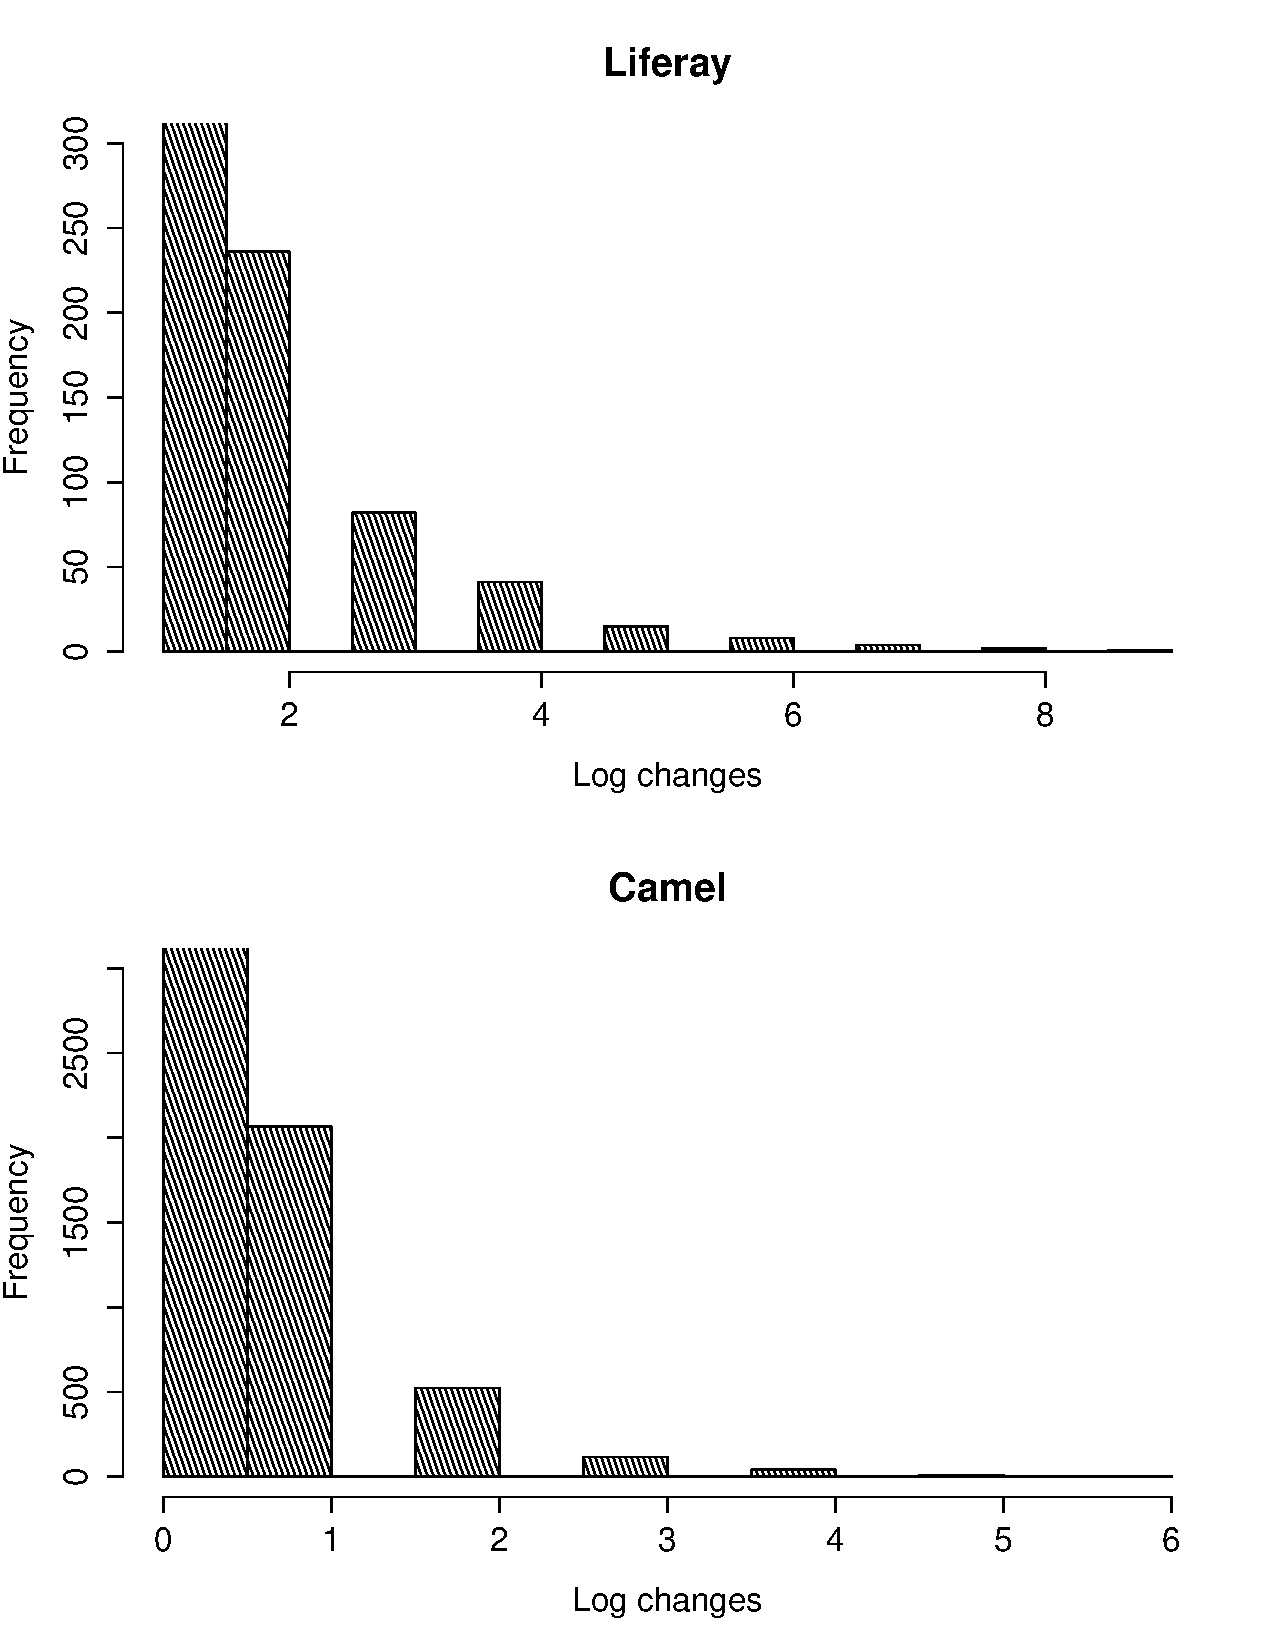
\includegraphics[width=0.7\linewidth]{RQ1_Liferay_Camel_Logchangefreq}
%	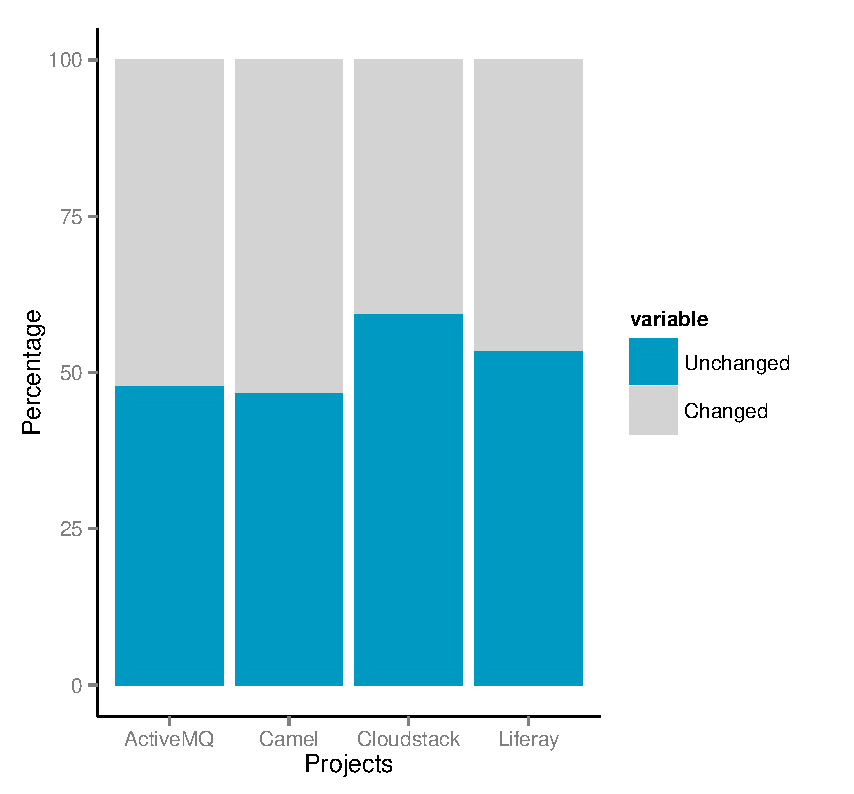
\includegraphics[width=0\linewidth]{Percentageofchanges}
%	\caption{Percentage of log changes in the studied projects.}
%	\label{fig:RQ1_Liferay_Camel_Logchangefreq}
%\end{figure}
%\
%\begin{table}[tb]
%	\centering
%	\smaller
%	\caption{{Distribution of changes to logging statemetns in the studied projects}
%	
%	\begin{tabular}{lrrrrrr}
%		\toprule
%		\textbf{Project} & \textbf{Min} & \textbf{1st Qu} & \textbf{Median} & \textbf{Mean} & \textbf{3rd Qu} & \textbf{Max} \\
%		\midrule
%		ActiveMQ   & 1   & 2      & 7      & 9    & 14     & 37  \\
%		Camel      & 1   & 1      & 2      & 4    & 5      & 117 \\
%		Cloudstack & 1   & 1      & 3      & 17   & 14     & 390 \\
%		Liferay    & 1   & 1      & 1      & 7    & 1      & 130\\
%		\bottomrule
%	\end{tabular}
%	\label{tba:frequencyofLogchanges}
%\end{table}

\begin{table}[tb]
	\centering
	\smaller
	\caption{Distribution of changes to logging statemetns in the studied applications}
	
	\begin{tabular}{lrr}
		\toprule
		\textbf{Application} & Unchanged logging  & {Changed logging } \\ 	
			& statements & statements\\
		\midrule
		ActiveMQ   &71.9 \%   & 28.0 \%     \\
		Camel      & 64.79 \%  & 35.20 \%    \\
		Cloudstack & 55.41 \%   & 44.58 \%    \\
		Liferay    & 78.7 \%  & 21.2 \%  \\
		\bottomrule
	\end{tabular}
	\label{tba:summaryofnewLogchange}
\end{table}

<<<<<<< HEAD
	\subfloat{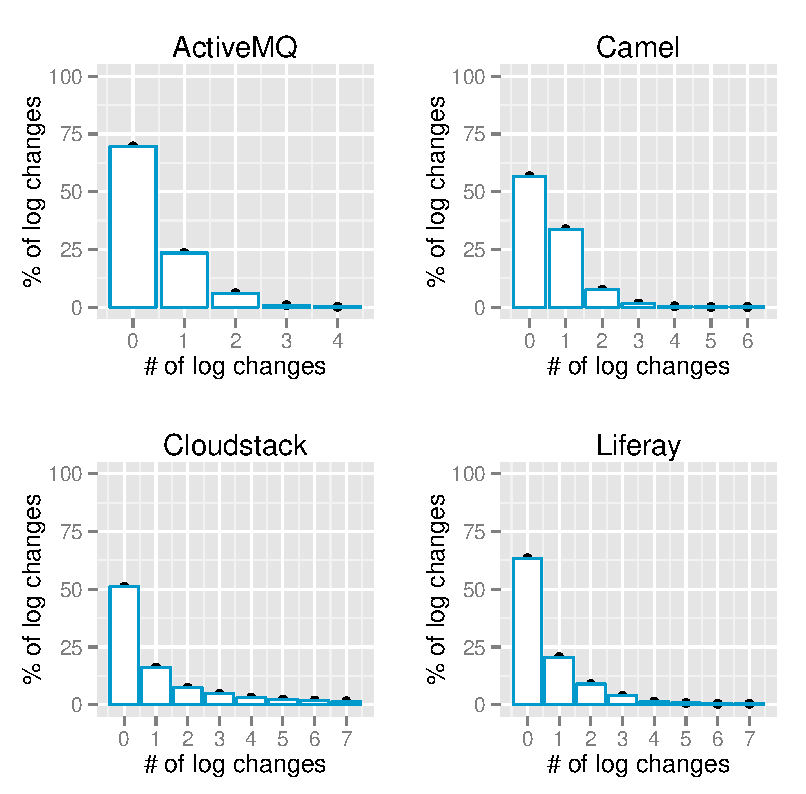
\includegraphics[height=.7\linewidth]
		{frequencyofLogchanges}\label{fig:Feq} }
	
	%	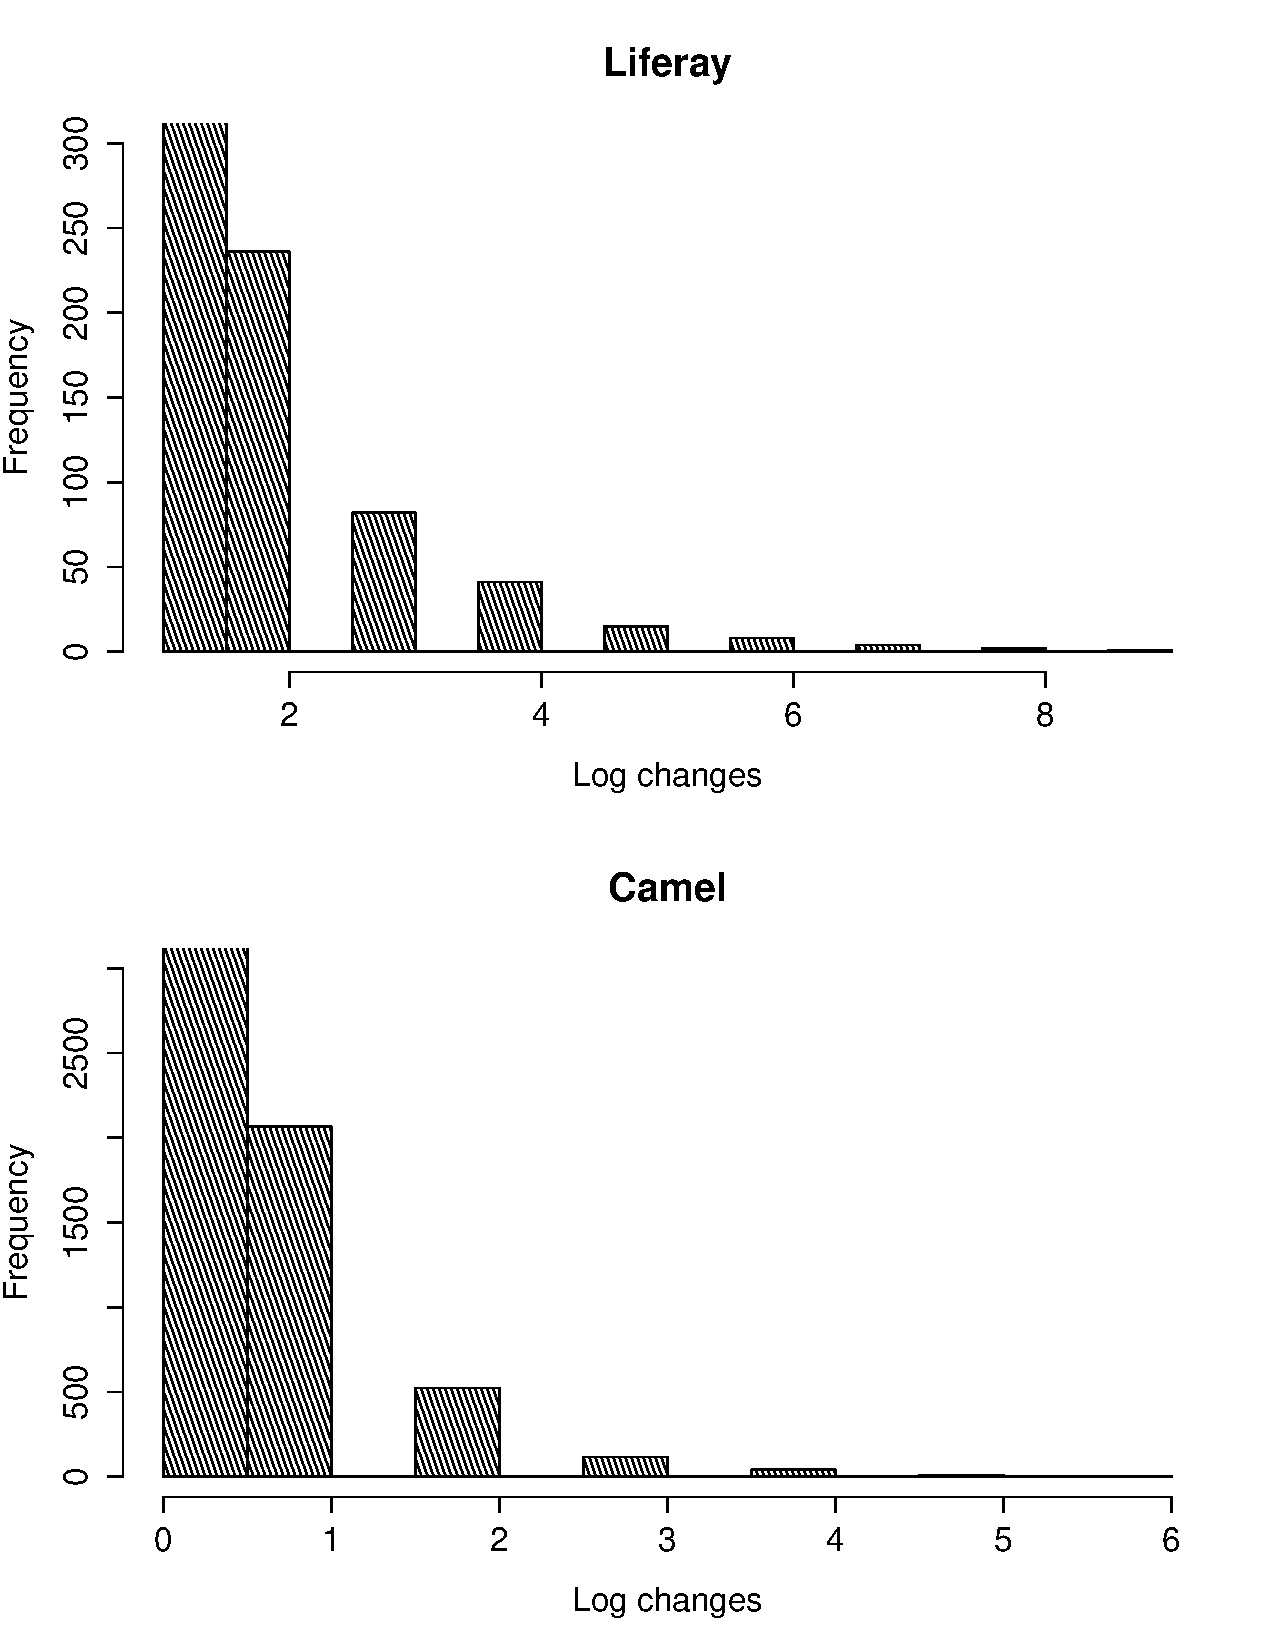
\includegraphics[width=0.7\linewidth]{RQ1_Liferay_Camel_Logchangefreq}
%	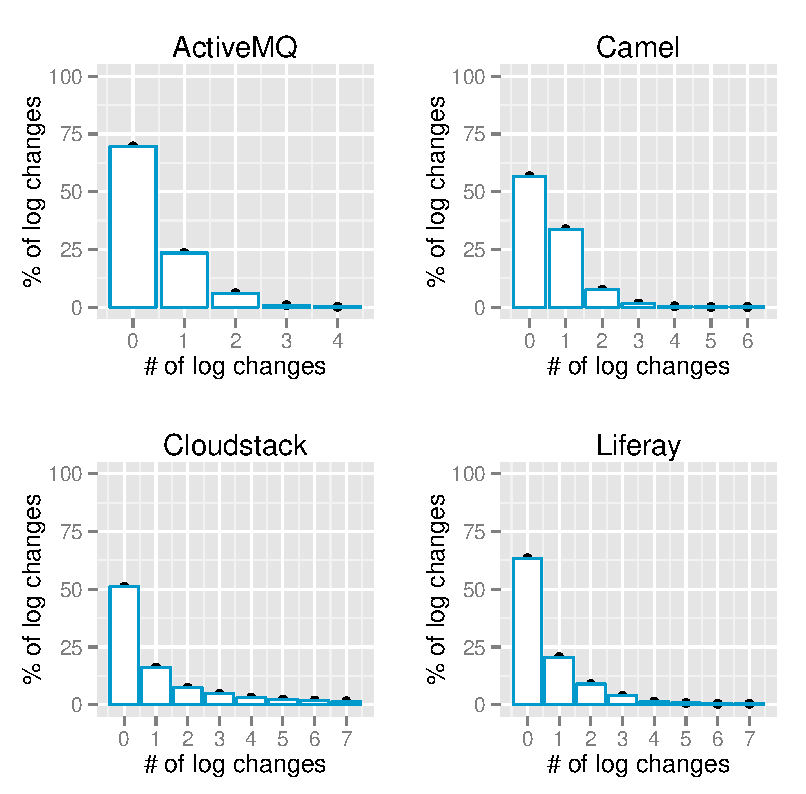
\includegraphics[width=0.9\linewidth]{frequencyofLogchanges}
	\caption{\ian{DELETE}Distribution of changes to logging statemetns in the studied projects	} 
	\label{fig:frequencyofLogchanges}
\end{figure}
=======
>>>>>>> c81afe5aab4af1198487f4494a3314e260e9fd43


%\begin{figure}[tb]
%	
%	\centering
%%	\captionsetup{justification=centre}
%	
%%		\subfloat[Percentage of log changes]{\includegraphics[width=0.5\linewidth]
%%			{Percentageofchanges}\label{fig:percentage} }
%
%	\subfloat{\includegraphics[height=.7\linewidth]
%		{frequencyofLogchanges}}
%	
%	%	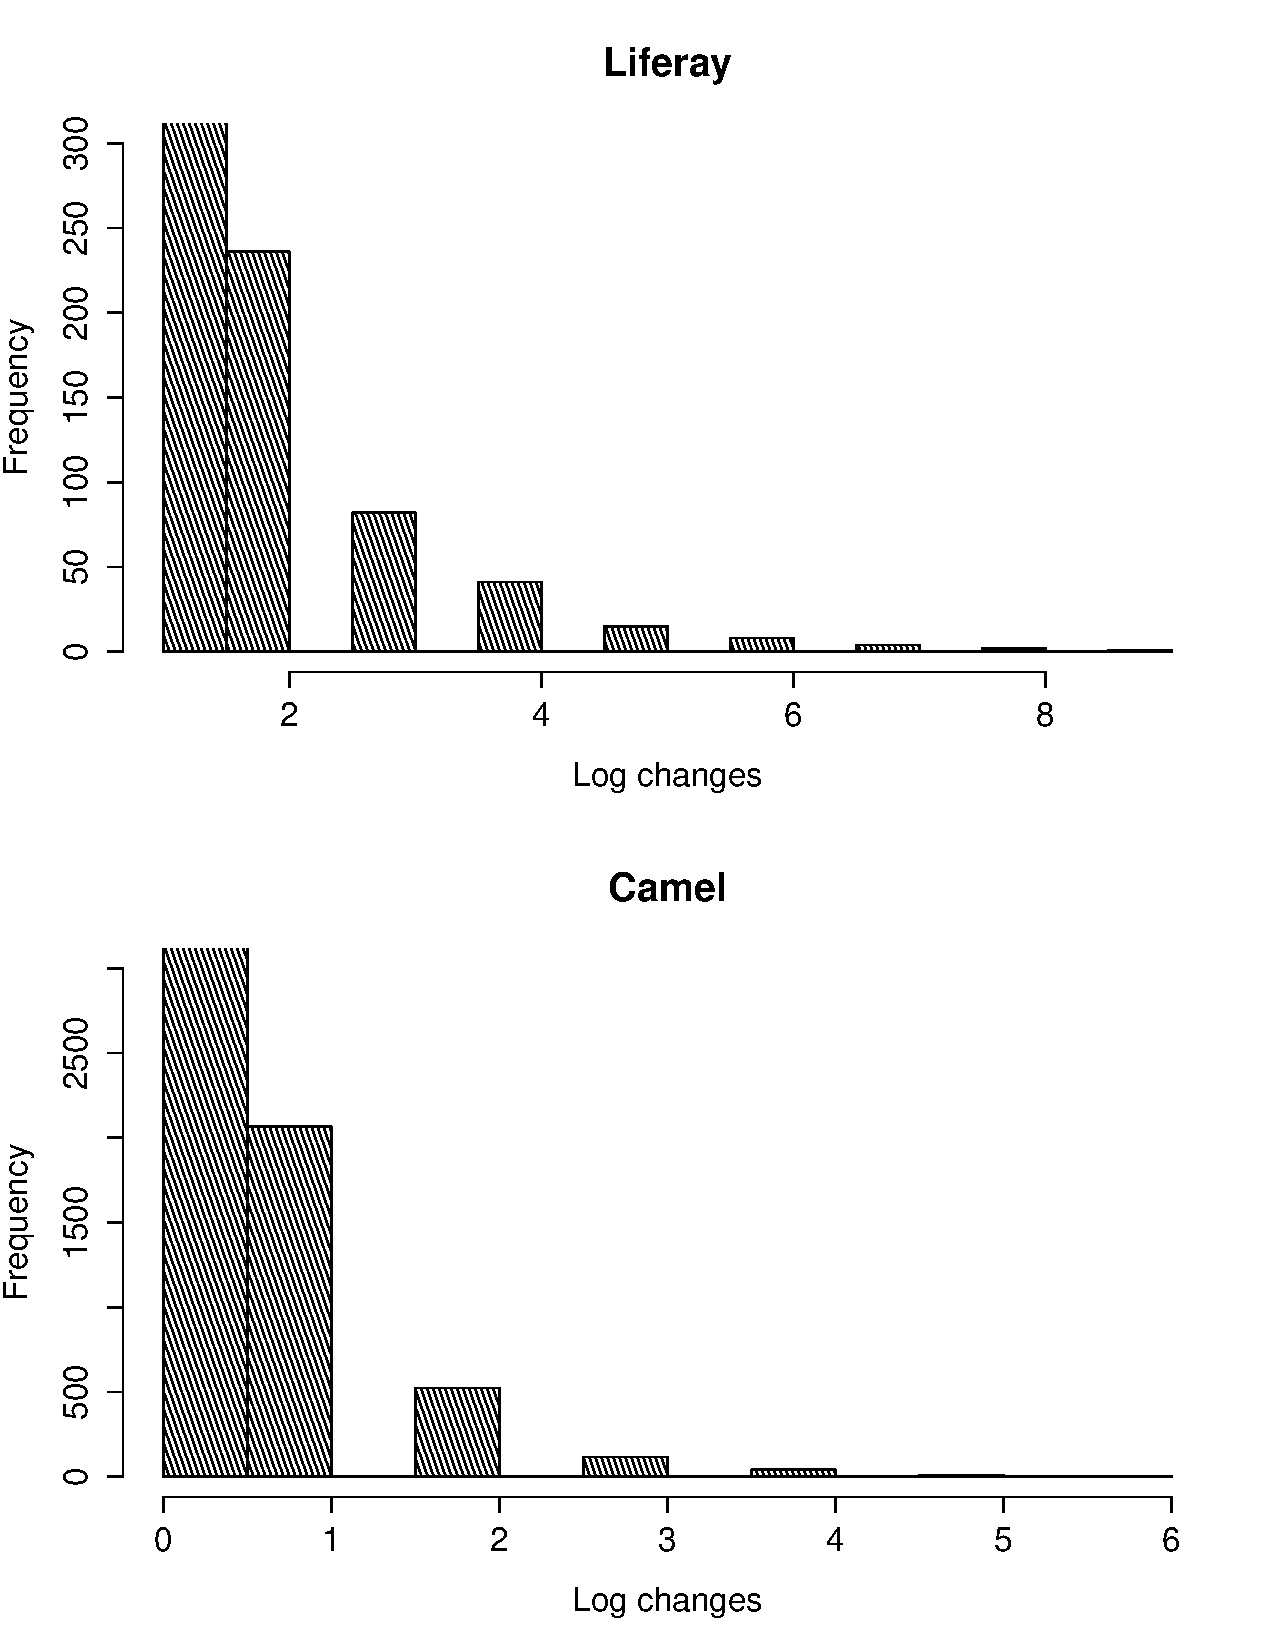
\includegraphics[width=0.7\linewidth]{RQ1_Liferay_Camel_Logchangefreq}
%%	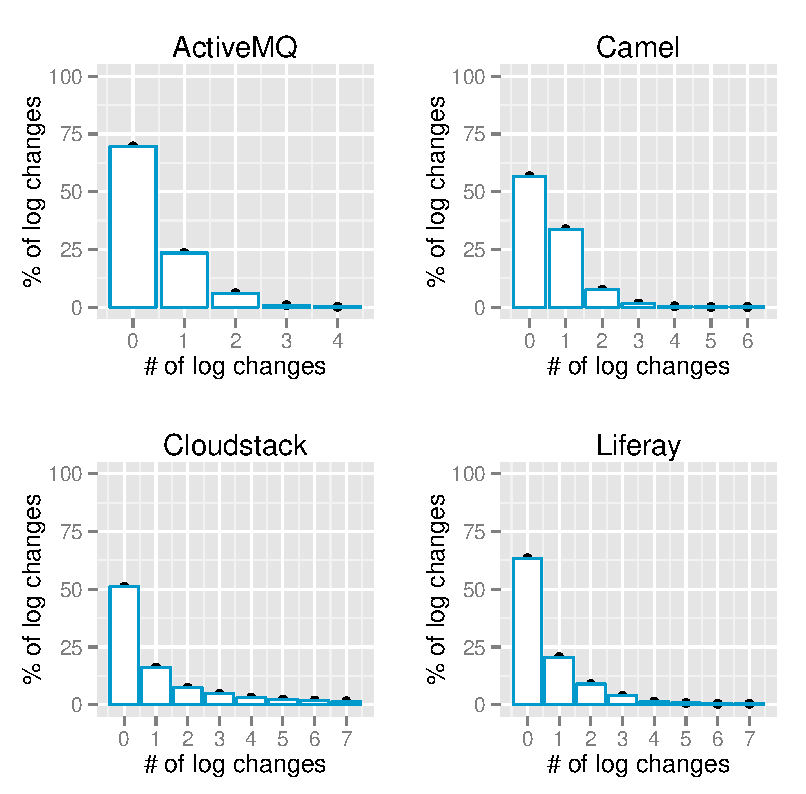
\includegraphics[width=0.9\linewidth]{frequencyofLogchanges}
%	\caption{Distribution of changes to logging statemetns in the studied projects	} 
%	\label{fig:frequencyofLogchanges}
%\end{figure}
%


%To find how frequently logs change, we conduct a quantitative analysis on the studied systems. We use the tracked log data for each studied system as explained in Section~\ref{Methodology}. From each project, we select a random sample with 95\% confidence interval. We follow the same iterative process as in prior research~\cite{IanIcesm} to find how frequently logs change in our studied systems. 





%\begin{figure}[tb]
%	
%	\centering
%	%	\subfloat{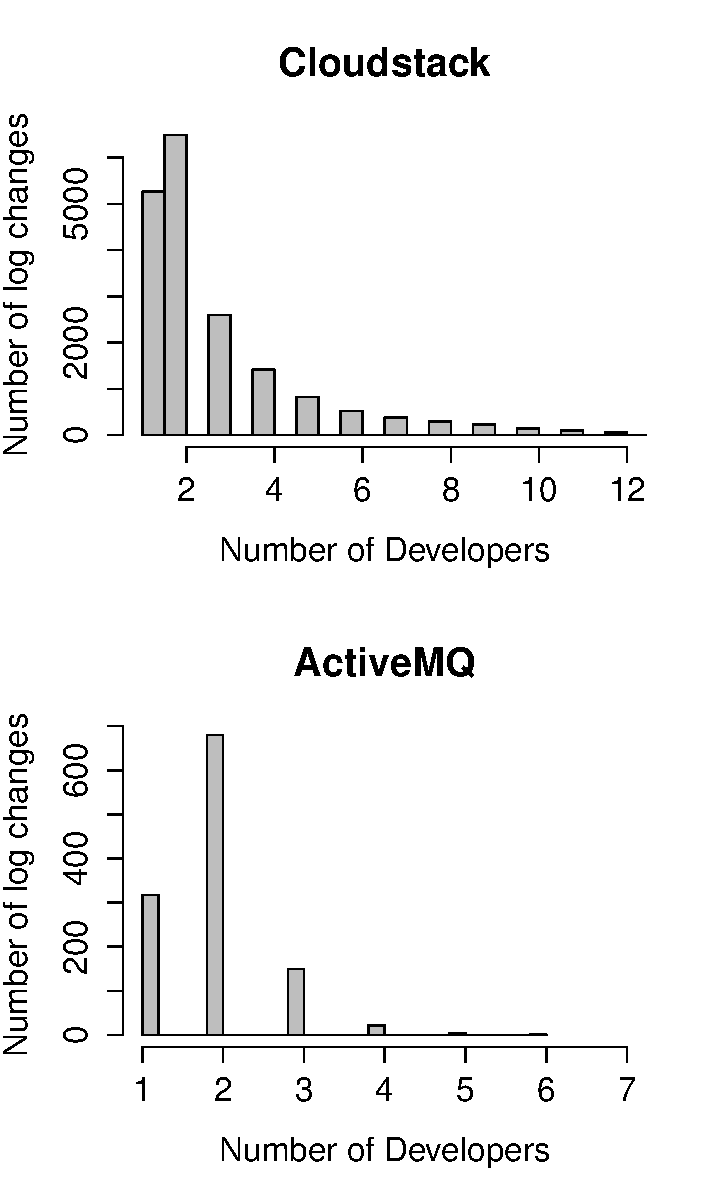
\includegraphics[width=0.5\linewidth]{CA_numberofDevelopers}\label{fig:f1}}
%	%	\hfill
%	\subfloat{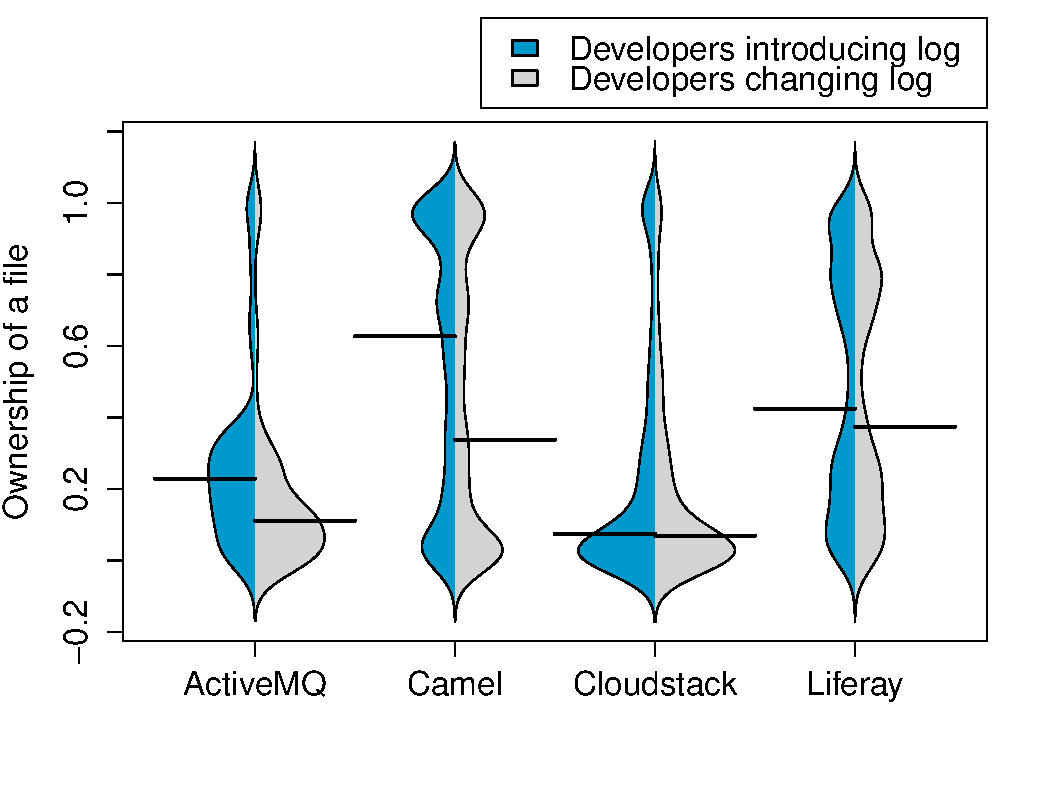
\includegraphics[width=1\linewidth]{ChangedvsChangesorNot}\label{fig:f2}}
%	\caption{Distribution of file ownership against developers introducing the log vs developers changing the log.}
%	\label{fig:ChangedvsChangesorNot}
%\end{figure}



%\begin{figure}[tb]
%	
%	\centering
%	%	\subfloat{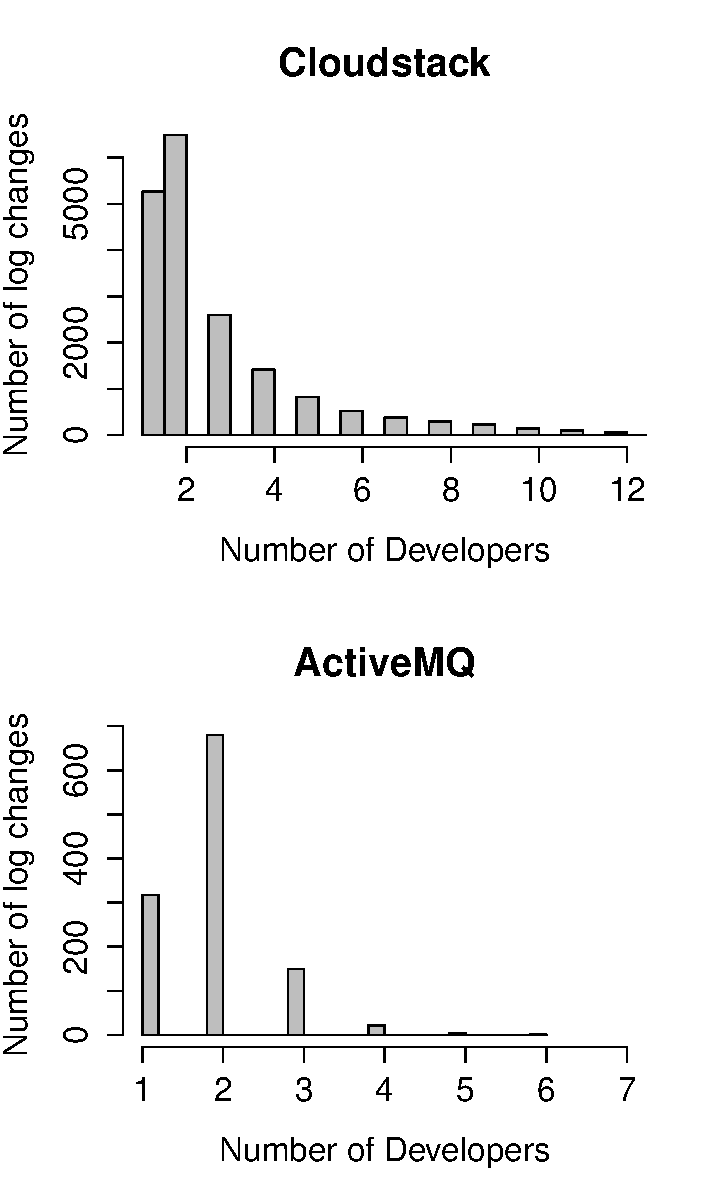
\includegraphics[width=0.5\linewidth]{CA_numberofDevelopers}\label{fig:f1}}
%	%	\hfill
%	\subfloat{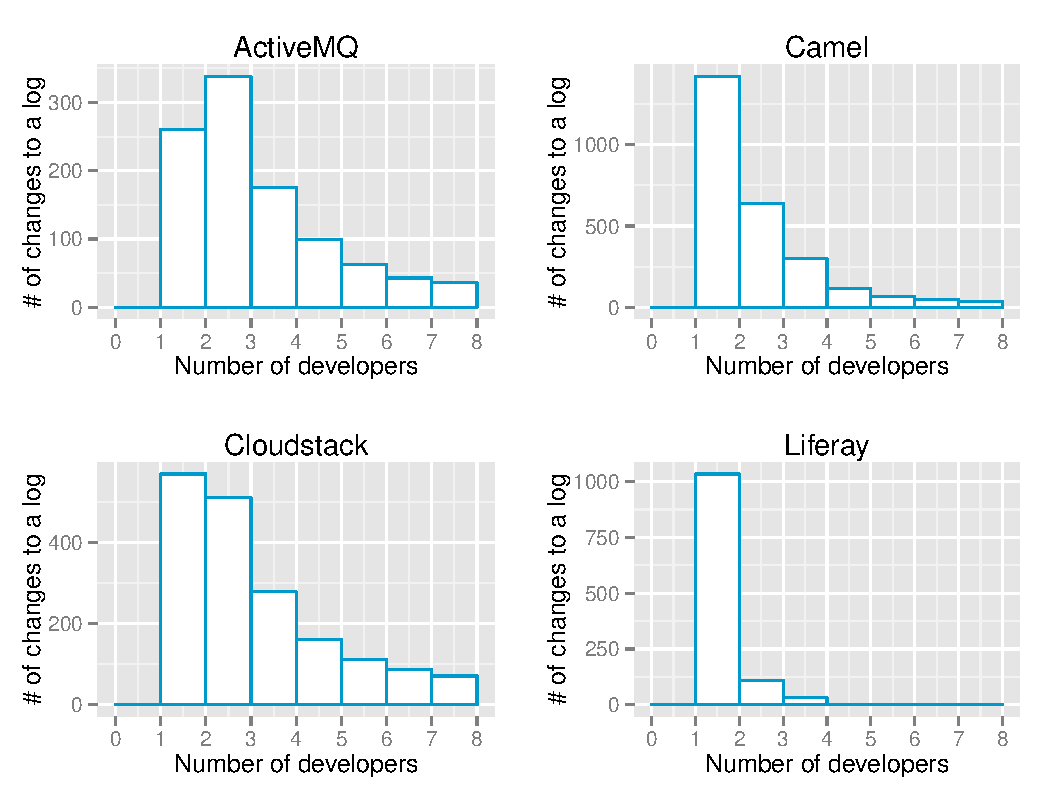
\includegraphics[width=1\linewidth]{NumberofDevelopers}\label{fig:f2}}
%	\caption{Distribution of the number of developers responsible
%		for changing a log.}
%	\label{fig:NumberofDevelopers}
%\end{figure}





\subsection{Results }

\begin{figure}[tb]
	
	\centering
	%	\captionsetup{justification=centre}
	
	%		\subfloat[Percentage of log changes]{\includegraphics[width=0.5\linewidth]
	%			{Percentageofchanges}\label{fig:percentage} }
	
	\subfloat{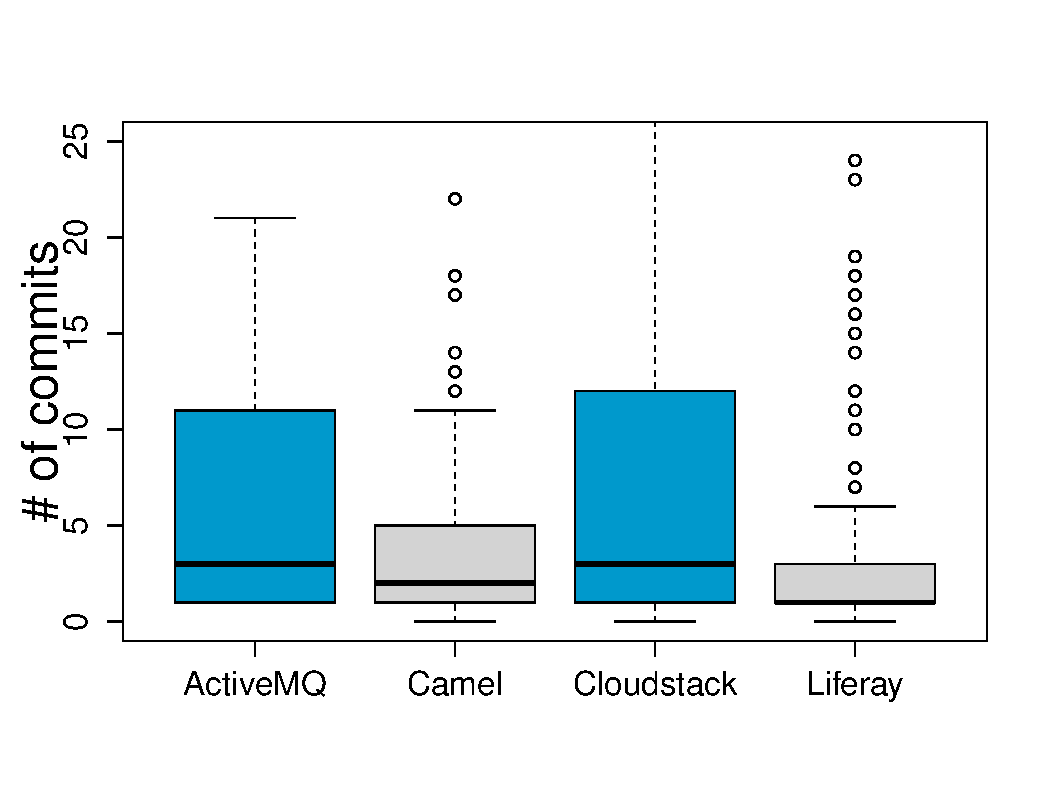
\includegraphics[height=.6\columnwidth,width=0.9\columnwidth,trim={0 1.5cm 0 2cm},clip]
		{NumberofCommits}}
	
	%	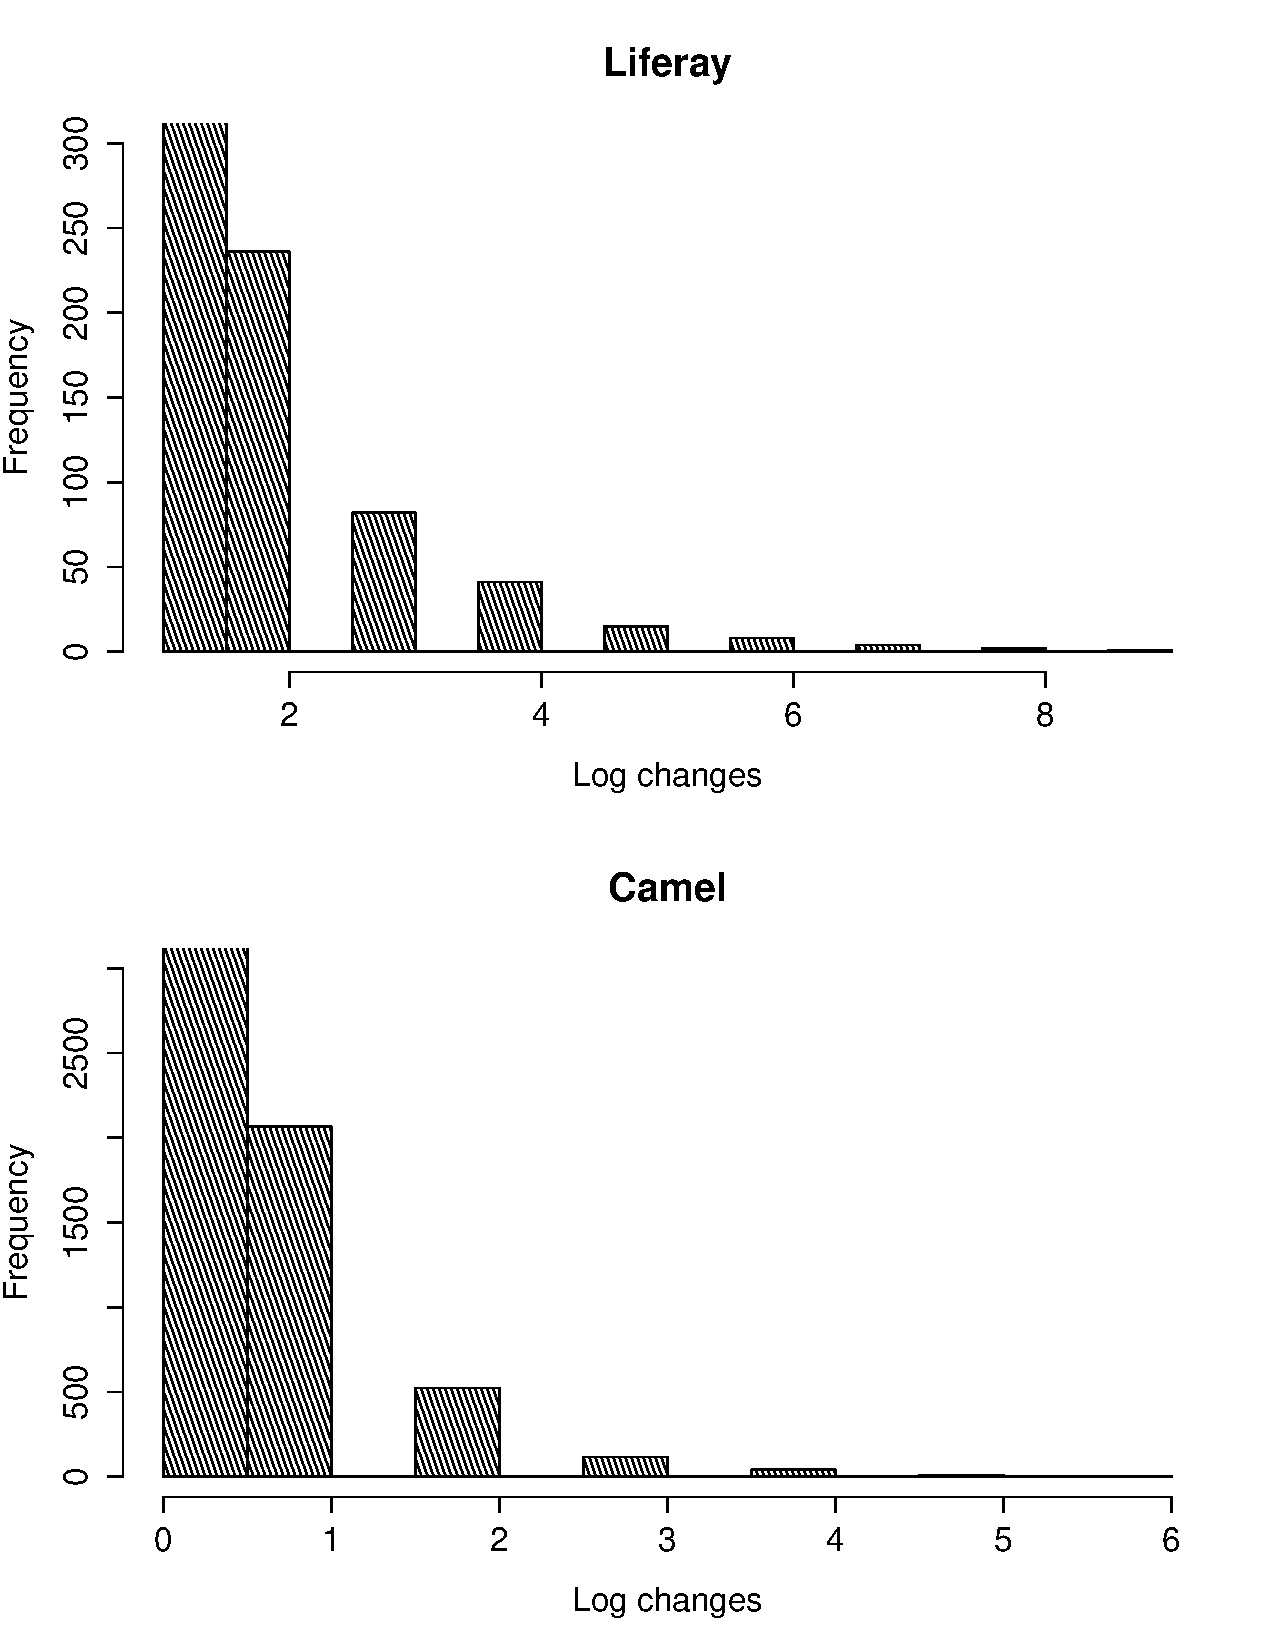
\includegraphics[width=0.7\linewidth]{RQ1_Liferay_Camel_Logchangefreq}
	%	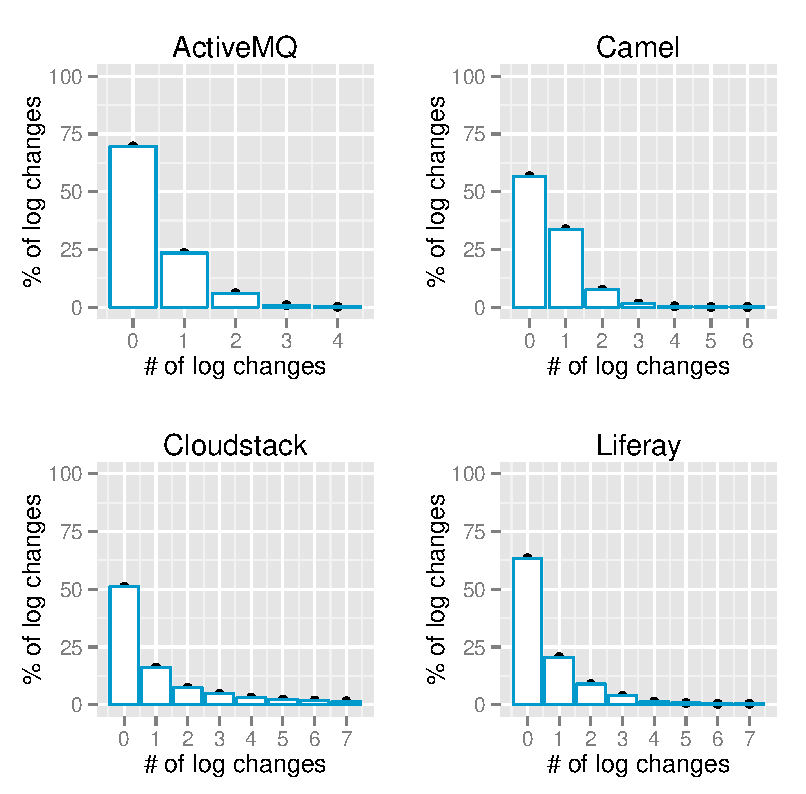
\includegraphics[width=0.9\linewidth]{frequencyofLogchanges}
	\caption{Number of commits before an added logging statement is changed in the studied applications } 
	\label{fig:NumberofCommits}
\end{figure}
\begin{figure}[tb]
	\setlength{\belowcaptionskip}{-10pt}
	\centering
	%	\captionsetup{justification=centre}
	
	%		\subfloat[Percentage of log changes]{\includegraphics[width=0.5\linewidth]
	%			{Percentageofchanges}\label{fig:percentage} }
	
	\subfloat{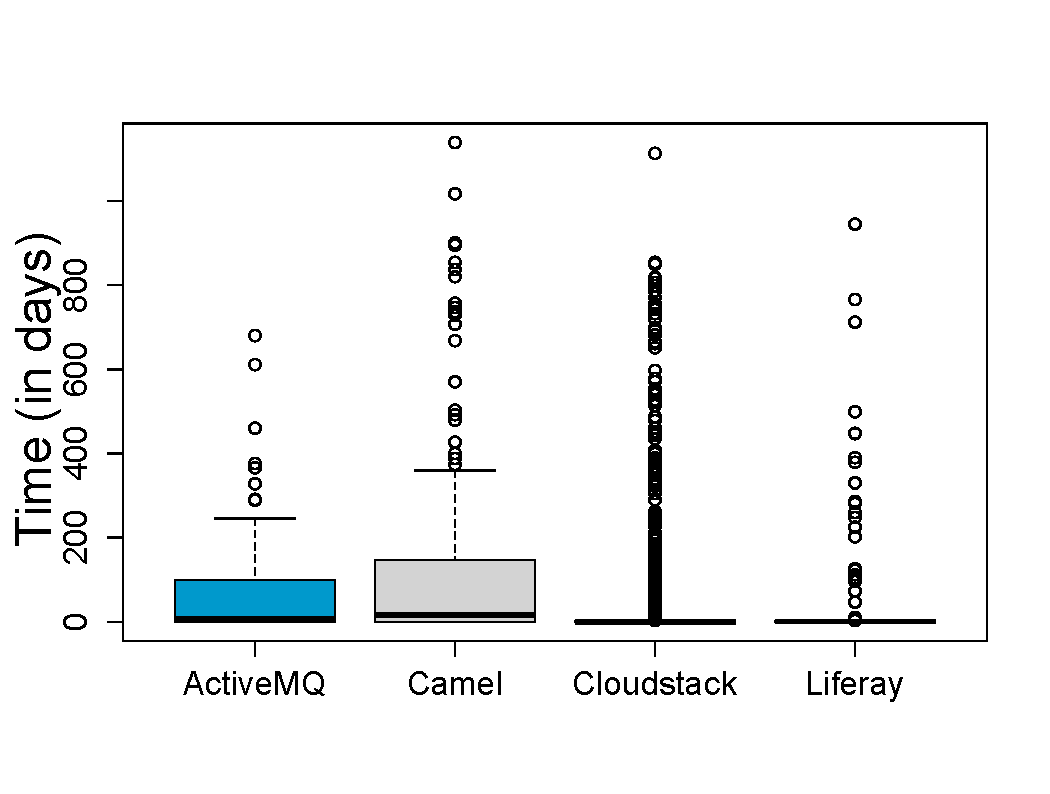
\includegraphics[height=.6\columnwidth,width=0.9\columnwidth,trim={0 1.5cm 0 2cm },clip]
		{Daysbeforechange}}
	
	%	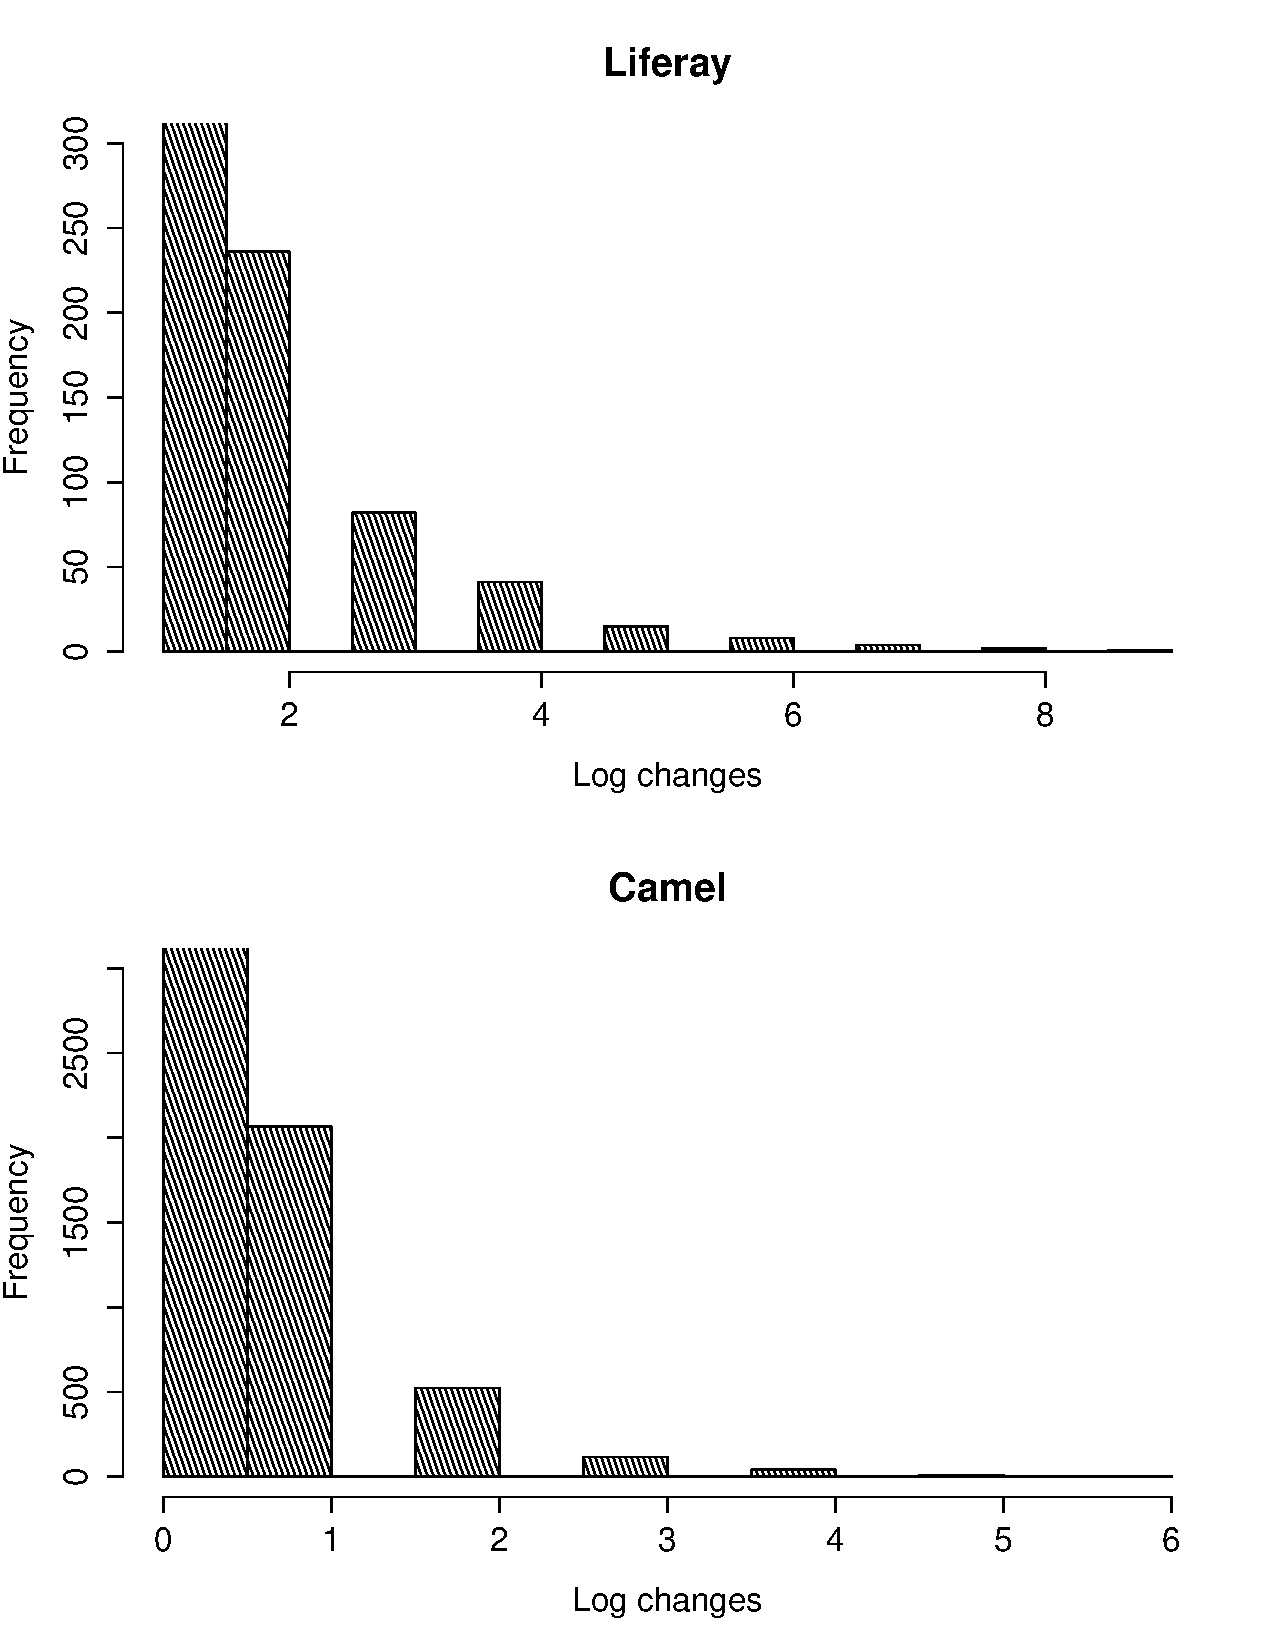
\includegraphics[width=0.7\linewidth]{RQ1_Liferay_Camel_Logchangefreq}
	%	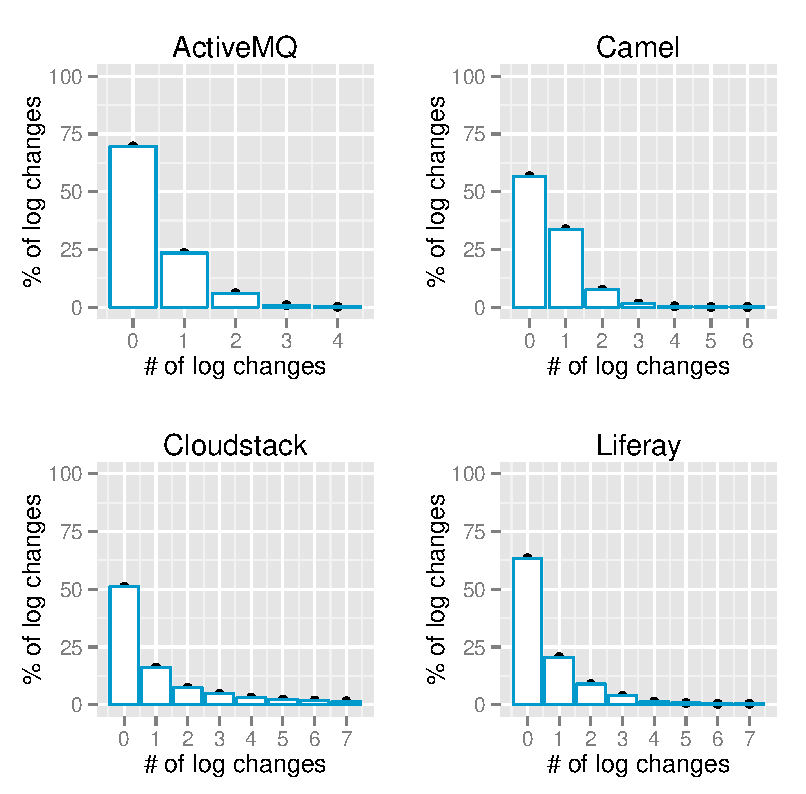
\includegraphics[width=0.9\linewidth]{frequencyofLogchanges}
	\caption{Number of days before an added logging statement is changed in the studied applications } 
	\label{fig:numberofdays}
\end{figure}

%

%\subsubsection*{C.1. Change frequency}
%<<<<<<< HEAD
%\hypobox {Developers change 20\%-45\% of the logging statements across our studied applications. }
%Figure~\ref{fig:frequencyofLogchanges} shows the percentage of logging statement changes in each of the studied application. This shows that logging statements change extensively throughout the lifetime of an project which can affect the log processing tools.
%=======
<<<<<<< HEAD
\hypobox {Developers change 25\%-45\% of the logging statements in the studied applications. The median number of days between the addition of a logging statement and its first change is between 1 and 17.}
Figure~\ref{fig:frequencyofLogchanges} shows the percentage of logging statement changes in each of the studied application. We observe that A\%, B\%, C\% and C\% of the logging statements are changed in ActiveMQ, Camel, Cloudstack and Liferay, respectively, during their lifetime\ian{add the number}. This shows that logging statements change extensively throughout the lifetime of a project, which can affect log processing tools.
=======
\hypobox {Developers change 25\%-45\% of the logging statements across our studied applications. The median number of days between the addition of a logging statement and its first change is between 1 and 17.}
Table~\ref{tba:summaryofnewLogchange} shows the percentage of logging statement changes in each of the studied application. We observe that in Liferay 25\%, while in Cloudstack 45\% of the logging statements changes. This shows that logging statements change extensively throughout the lifetime of an application, which can affect log processing tools.
>>>>>>> c81afe5aab4af1198487f4494a3314e260e9fd43
%>>>>>>> 5547d3195c6b4fa9e75d8d7ea7226c9867cdee66

%\begin{table}[t]
%	\centering
%	\smaller
%	\caption{Days between the addition and first change of a logging statement\cp{BOXPLOT}}
%	
%	\begin{tabular}{lrrrrrr}
%		\toprule
%		\textbf{Project} & \textbf{Min} & \textbf{1st Qu} & \textbf{Median} & \textbf{Mean} & \textbf{3rd Qu} & \textbf{Max} \\
%		\midrule
%		ActiveMQ   & 1  & 1      & 7     & 86    & 99     & 680  \\
%		Camel      & 1   & 1      & 17      & 127    & 145      & 1139 \\
%		Cloudstack & 1   & 1      & 1      & 46   & 1     & 1113 \\
%		Liferay    & 1   & 1      & 2     & 34    & 2     & 945\\	
%		\bottomrule
%		
%	\end{tabular}
%	\label{tba:summaryofnewLogCodechange}
%\end{table}


%\textbf{We find that 12\%-40\% of the logging statement changes, are due to the added logging statements which change.} 
<<<<<<< HEAD
From Figure~\ref{fig:numberofdays}, we observe that 75\% of the changes to logging statements are done within 145 days after the log is added. In fact, the largest median number of days between the addition of a logging statement and its first change is 17 in our studied projects. This number shows that, all too often, the changes to logging statements happen in a short time after the logging statement being added. Hence, it is important for developers of log processing tools to not depend on logging statements that are likely to change, as this dependency will require additional maintenance within a short time.
=======
From Figure~\ref{fig:numberofdays}, we observe that 75\% of the changes to logging statements are done within 145 days after the log is added. In fact, the largest median number of days between the addition of a logging statement and its first change is 17 in our studied applications. This number shows that a large part of the logging statements that will change will do so in a short time. Hence, it is important for developers of log processing tools to not depend on logging statements that are likely to change, as this dependency will require additional maintenance within a short time.
>>>>>>> c81afe5aab4af1198487f4494a3314e260e9fd43

% that any log processing tool utilizing a logging statement introduced in the previous releases, is more susceptible to breakage by changes to the added logging statement.  

% that upto 75\% of logging statement changes occur within 4 months of across all our applications. 

% find that over 75\% of the changes occur within 4 months of addition. 

% suggests tha which are added 

%\textbf{75\% of the new logs which change, are changed within 15 commits since their addition.} From Table~\ref{tba:summaryofnewLogchange}, we find that majority, i.e., 75\% are changed within 15 commits since addition.  We also find that the median code churn during these log changes is less than 50 lines of code in three of the studied projects as seen in Table~\ref{tba:summaryofnewLogCodechange}. This suggests that the log changes are more likely to be changed due to rewording changes rather than major changes to the added feature. This means that new logs which are introduced prior to 15 commits in the studied projects, are less likely to break the log processing tools which might depend on them. 


%\textbf{25\% of the new logs which change, are changed after 15 commits since their addition.} From Table~\ref{tba:summaryofnewLogchange}, we find 25\% of the new logs added are changed after 15 commits since their addition. We also find that the code churn during these log changes is more than 150 lines of code in three of the studied projects as seen in Table~\ref{tba:summaryofnewLogCodechange}. This suggests that these log changes are more likely to be changes to the feature rather than rewording changes, and are more likely to affect the log processing tools. 

%This also means that the remaining 25\% of log changes might break the log processing tools which might rely on them, as they are changed much later. 



%rewording or after-thoughts rather than change of feature.

% This short time between addition and log change suggests that log change are more likely to be rewording or after-thoughts rather than change of feature. This is seen in Table~\ref{tba:summaryofnewLogCodechange} where in three of the projects, the code churn is less than 50 lines of code for 50\% of the new logs which are changed before 15 commits since addition. 



%We find that logs are added throughout the lifetime of an project and these logs are changed within 

%, the logs added near the end of our study time-frame can change but will not be considered in our analysis. We find that a new log is changed between 37 to 390 commits within our projects as seen in Table~\ref{tba:summaryofnewLogchange}. To eliminate such logs, we find the maximum number of commits before a newly added log is changed within the studied projects and exclude all new logs added before that many commits from our analysis. 


%From Table~\ref{tba:summaryofnewLogchange}, we see that the maximum value varies greatly within the studied projects and we exclude all newly added logs into the project before the 
 
%as shown in Figure~\ref{fig:RQ1_Liferay_Camel_Logchangefreq}. 



%Based on frequency of changes, we categorize logs into 3 categories namely: a) Frequently Changed, b) Changed and c) Never Changed as shown in Table~\ref{tba:logchangeDistribution}. If a log is changed more than four times it is categorized as `Frequently Changed'. If it is changed 1 to 3 times it is categorized under `Changed' and if it did not change it is categorized under `Never Changed'. We select four as the threshold as we observe that majority of logs only have 1 to 2 changes as seen in Figure~\ref{fig:RQ1_Liferay_Camel_Logchangefreq}. We see that the majority of logs never change in Liferay and the majority of logs in ActiveMQ and CloudStack are changed atleast once. This may be because Liferay has fewer logs per source code file (i.e., lower log density) when compared to ActiveMQ and CloudStack as seen in Table~\ref{tba:overviewsystems}. 


%\subsubsection*{C.2. Developer impact}
%After identifying the frequency of changes within the studied projects, we find the number of the developers responsible for the log changes and also if they own the file which contains the log. We use the developer name available from the `git log' to count the number of developers who change a log. To decide whether a developer owns a file we calculate the ratio of number of lines written by him to the total lines of code using the `blame' command available in Git. Since \emph{blame} only shows the changes made to a file in the last commit, to calculate the contribution of a developer to a file we recursively look at changes made in previous commits by that developer. We use the \emph{blame} to calculate the contribution at each commit and take the mean contribution across all commits to find his ownership of a file.

%we obtain all the the commits made to a file and calculate th



%\hypobox{Logs which change are introduced by developers who have little ownership over the file.} 
%Figure~\ref{fig:ChangedvsUnchangedlogs} shows that in Camel, Cloudstack and Liferay, the logs which change are more likely to be introduced by developers who have less ownership on the files, than logs which are never changed. This suggests that logs can be introduced by non-owners of a file, which leads to logs being changed later. 

%We see that logs are changed by developers who have lesser ownership over the 
%file than the developers who introduce the log.

%We see thats logs are also changed by developers who have lesser ownership than the ones introducing them. Figure~\ref{fig:ChangedvsChangesorNot} shows that in all the studied projects the logs are more likely to be changed by developers who have lesser ownership on the file than the developers who introduce the log. These results suggest that logs are readily changed by developers who access the file but do not have strong ownership characteristics.   



%These results suggest that logs are readily changed by developers who access the file but do not have strong ownership characteristics.

%Figure~\ref{fig:ChangedvsChangesorNot} shows that in all the studied


 

% which change are introduced by developers who have less ownership on files than the developers who introduce the log.
 
%  We also find that in one of the studied projects the majority of logs are changed by two or more developers as seen in Figure~\ref{fig:NumberofDevelopers}. 

% we see that in two of the studied systems, a single developer is responsible for majority of the log changes. 

%This suggests that logs can be 
% do not have strong ownership characteristics and can be changed by developers than one introducing the logs.

%\hypobox {45\%-55\% of the logs are changed atleast once in the studied projects. We find that over 51\% of the changes are made to the static content, variable content and log level. We also find that logs are changed by developers who have little ownership of the file and in two of the projects we find the majority of logs are changed by two or more developers.}

%When logs are changed, they can be changed in five possible ways namely:
%\begin{enumerate}
%	
%	\item { \textbf{Log relocation:} } The log is kept intact but moved to a different location in the file because of context changes (code around the log is changed).
%	
%	\item \textbf{Text change:} The text (i.e., static content) of log is changed. 
%	
%	\item\textbf{Variable change:} One or more variables in the log are changed (added, deleted or modified).
%	
%	\item \textbf{Change of log level:} The verbosity level of a log is changed.
%	
%	\item  \textbf{Text and variable change:} Both text and variables in the logs are changed. This is generally done when developers provide more context information, i.e, text and add/modify the relevant variables in a log.
%	
%\end{enumerate}
%
%%for several reasons. To understand the different types of log changes we perform a manual analysis on the changed logs. We select a random sample from each project such that the sample achieves 95\% confidence interval. After identifying the different types of log changes we automate the process of identification using our scripts. Figure~\ref{fig:Flowchart2} highlights the process of categorizing the log changes. For example,consider the logs shown below. 


%We see that there can be only four possible ways in which developers change logs namely:
%
%To automate the process of categorizing log changes into these categories, we first remove the logging method (i.e, LOG) and the log level (i.e, info) from the logs. We then compute the \textsl{Levenshtein ratio} between each term within the parentheses. In the example below we find that `+ Integer.toString(listenPort)' has \textsl{Levenshtein ratio} of 1, implying they are identical and the \textsl{Levenshtein ratio} between `starting HBase HsHA Thrift server on' and `starting HBase' is 0.56. This suggests there is some similarity between the two strings and the variable is constant which implies its a text change. (Figure~\ref{fig:Flowchart2} highlights the process of categorizing the log changes.
%
%\hypobox {+ LOG.info(``starting HBase HsHA Thrift server on " + Integer.toString(listenPort)); }
%
%\hypobox {- LOG.info(``starting HBase " + implType.simpleClassName() +`` server on " + Integer.toString(listenPort)); }



% ownership of file using the `blame' command available in git i.e.., if two developers are responsible for a file, but one has written 100 of the 150 lines of code, we calculate his 
%\begin{enumerate}
%	
%	\item { \textbf{Log relocation:} } The log is kept intact but moved to a different location in the file because of context changes (code around the log is changed).
%	
%	\item \textbf{Text change:} The text (i.e., static content) of log is changed. 
%	
%	\item\textbf{Variable change:} One or more variables in the log are changed (added, deleted or modified).
%	
%	\item \textbf{Change of log level:} The verbosity level of a log is changed.
%	
%	\item  \textbf{Text and variable change:} Both text and variables in the logs are changed. This is generally done when developers provide more context information, i.e, text and add/modify the relevant variables in a log.
%	
%\end{enumerate}
% 

%\noindent \textbf{Results}


%{\suhas{ I have question Can i tell here that in RQ2 we find log density to be imporatnt factor in stability of logs ?? }}

% are project layer software which  rely less on logs as they are middle-ware/project software, whereas ActiveMQ and CloudStack are service software.




%From manually analyzing the changed logs, we identify five types of log changes (i.e., changes to verbosity levels, log context, logged variables, both context and variable and relocation of log).  Table~\ref{tba:logtype} shows their distributions. When there is overlapping of the different types of log changes, we categorize them as newly added log and track changes made to it.

%	We find that about 3-11 \% of logs are changed frequently. This suggests that log processing tools which run on these systems need constant maintenance from developers

